\documentclass[11pt]{article}
\usepackage[T1]{fontenc}
\usepackage{lmodern,microtype}
\usepackage[margin=1.05in]{geometry}
\usepackage{amsmath,amssymb,amsthm,mathtools}
\usepackage{booktabs}
\usepackage{tikz}
\usepackage[hidelinks]{hyperref}
\usepackage[nameinlink,noabbrev]{cleveref}
\usepackage{enumitem}
\setlist{itemsep=2pt,topsep=5pt}
\newtheorem{theorem}{Theorem}[section]
\newtheorem{proposition}[theorem]{Proposition}
\newtheorem{lemma}[theorem]{Lemma}
\newtheorem{corollary}[theorem]{Corollary}
\theoremstyle{remark}
\newtheorem{remark}[theorem]{Remark}
\newcommand{\R}{\mathbb R}
\newcommand{\E}{\mathbb E}
\newcommand{\eps}{\varepsilon}
\DeclareMathOperator{\tr}{tr}
\DeclareMathOperator{\Var}{Var}
\DeclareMathOperator{\Sym}{Sym}
\DeclareMathOperator{\supp}{supp}
\numberwithin{equation}{section}
\allowdisplaybreaks[1]
\hypersetup{pdftitle={The logarithmic Brunn--Minkowski conjecture},pdfauthor={OpenAI}}
\pdfinfoomitdate=1
\pdftrailerid{}
\pdfsuppressptexinfo=15
\title{The logarithmic Brunn--Minkowski conjecture}
\author{OpenAI}
\date{September 23, 2026}
\begin{document}
\maketitle
\begin{abstract}
We prove the logarithmic Brunn--Minkowski conjecture for arbitrary
origin-symmetric convex bodies in every dimension. The theorem also gives
the symmetric $L_p$ Brunn--Minkowski inequality for every $0<p<1$.
Combined with Saroglou's transfer theorem and a support-subspace reduction,
it yields the logarithmic inequality for every even log-concave Radon
measure and the scalar-dilation $(B)$-conjecture.
\end{abstract}
\tableofcontents

\section{Introduction}
\label{sec:introduction}

A convex body in $\R^n$ is a compact convex set with nonempty interior.
If $K=-K$, then $0$ lies in its interior.
Its support function is
\[
 h_K(u)=\max_{x\in K}\langle x,u\rangle,\qquad u\in S^{n-1}.
\]
For an origin-symmetric body this function is strictly positive.
For a positive continuous function $f$ on the unit sphere, its
\emph{Wulff body} is
\[
 \mathcal W[f]=\bigcap_{u\in S^{n-1}}
 \{x\in\R^n:\langle x,u\rangle\le f(u)\}.
\]
It is a convex body: it contains the ball of radius $\min f>0$ and
is contained in the ball of radius $\max f$. Write $|K|$ for
$n$-dimensional Lebesgue measure. Our main result is the following.

\begin{theorem}[Even logarithmic Brunn--Minkowski inequality]
\label{thm:main}
Let $n\ge1$ and let $K,L\subset\R^n$ be convex bodies satisfying
$K=-K$ and $L=-L$. For every $0\le\lambda\le1$,
\begin{equation}\label{eq:main}
 \left|\mathcal W[h_K^{1-\lambda}h_L^\lambda]\right|
 \ge |K|^{1-\lambda}|L|^\lambda.
\end{equation}
\end{theorem}

The interpolation in \eqref{eq:main} takes the geometric mean of the
support bounds before intersecting the half-spaces. This gives a
strengthening, in the symmetric setting, of the multiplicative form
of the classical Brunn--Minkowski inequality: the arithmetic--geometric
mean inequality gives
\[
 \mathcal W[h_K^{1-\lambda}h_L^\lambda]
 \subset (1-\lambda)K+\lambda L.
\]
In general $h_K^{1-\lambda}h_L^\lambda$ need not itself be a support
function. The intersection defining $\mathcal W$ is essential throughout
the argument.

For $0<p<1$, the $L_p$ interpolation replaces the geometric mean of the
support bounds by the weighted power mean
$((1-\lambda)h_K^p+\lambda h_L^p)^{1/p}$, still taking the Wulff body.
The logarithmic endpoint implies the full symmetric volume inequality in
this intermediate range. B\"or\"oczky, Lutwak, Yang and Zhang record
this monotone implication
\cite[equation~(1.10) and the following paragraph, p.~1977]{BLZY2012}.
The additive
volume-power form below follows by normalizing the bodies and reweighting
the interpolation parameter.

\begin{corollary}[Symmetric $L_p$ Brunn--Minkowski inequality]
\label{cor:lp}
Let $n\ge1$, let $K,L\subset\R^n$ be full-dimensional origin-symmetric
convex bodies, and let $0<p<1$. For every $0\le\lambda\le1$,
\begin{equation}\label{eq:lp}
 \left|\mathcal W\!\left[
  \bigl((1-\lambda)h_K^p+\lambda h_L^p\bigr)^{1/p}
 \right]\right|^{p/n}
 \ge (1-\lambda)|K|^{p/n}+\lambda|L|^{p/n}.
\end{equation}
\end{corollary}

The proof of Corollary~\ref{cor:lp} is given in
Section~\ref{subsec:lp-proof}.


The logarithmic volume theorem has a separate measure-theoretic consequence.
An even log-concave density has the form $e^{-V}$, where $V$ is an even
convex function with values in $\R\cup\{+\infty\}$; no probability
normalization is required. Saroglou proved that the Lebesgue inequality in
dimension $n$ implies the same Wulff inequality for every such density in
that same dimension \cite[Theorem~3.1]{Saroglou2016}.
Taking two scalar dilates of a single body then gives the $(B)$-conjecture:
for the measure $d\mu=e^{-V(x)}\,dx$ and every origin-symmetric convex body
$K$, the function $t\mapsto\mu(e^tK)$ is log-concave on $\R$
\cite[Corollary~3.2]{Saroglou2016}.
Section~\ref{sec:measure} applies this transfer and also treats even
log-concave Radon measures supported on proper subspaces.

\subsection*{Context and prior work}
Theorem~\ref{thm:main} resolves the origin-symmetric logarithmic
Brunn--Minkowski conjecture of B\"or\"oczky, Lutwak, Yang and Zhang
\cite[Problem~1.1]{BLZY2012}.
Stancu \cite[Theorem~2, p.~3264]{Stancu2018} announced the
all-dimensional logarithmic Minkowski inequality and explicitly concluded
the equivalent logarithmic Brunn--Minkowski inequality; the report deferred
details of the flow asymptotics.
The conjecture belongs to the $L_p$ Brunn--Minkowski theory initiated
by Firey's $p$-means of convex bodies
\cite{Firey1962} and developed by Lutwak through $L_p$ mixed volumes
and the $L_p$ Minkowski problem \cite{Lutwak1993}.
For $p>0$, the support bounds are interpolated by the weighted power
mean appearing in Corollary~\ref{cor:lp}; the geometric mean is
its limit as $p\downarrow0$. This endpoint has a particularly close
connection with cone-volume measures and the logarithmic Minkowski
problem. The cone-volume measure records the volumes of cones from the
origin to boundary patches, indexed by their outer normals. B\"or\"oczky, Lutwak, Yang and Zhang established the equivalence
between the corresponding logarithmic volume and mixed-volume inequalities
\cite[Lemma~3.2]{BLZY2012}; their subsequent work characterized which even
measures arise as cone-volume measures \cite[Theorem~1.1]{BLYZ2013}. The latter is an existence result,
separate from the volume inequality proved here.

Several important classes were established in earlier work.
B\"or\"oczky, Lutwak, Yang and Zhang proved the planar case
\cite[Theorem~1.3]{BLZY2012}.
Saroglou established the inequality and studied its equality cases for
bodies unconditional with respect to the same orthonormal basis, meaning that both bodies are invariant under
every coordinate sign change in that basis
\cite[Theorem~1.2]{Saroglou2015}.
The underlying volume inequality for coordinatewise products has antecedents
in Uhrin, Bollob\'as--Leader, and Cordero-Erausquin--Fradelizi--Maurey
\cite{Uhrin1994,BollobasLeader1995,CFM2004}; Saroglou connected this
product to the logarithmic combination. This argument uses the multiplicative
form of the Pr\'ekopa--Leindler inequality.
B\"or\"oczky and Kalantzopoulos extended the symmetry method to bodies
invariant under the same $n$ linear reflections whose fixed hyperplanes
intersect only at the origin \cite[Theorem~2]{BK2022}.
For unit balls of complex norms, Rotem derived the inequality from
Cordero-Erausquin's volume inequality for complex interpolation
\cite{Rotem2014,Cordero2002}.

A complementary approach studies the second variation of volume.
Colesanti, Livshyts and Marsiglietti established a local result near
Euclidean balls and developed infinitesimal formulations
\cite{CLM2017}. Kolesnikov and Milman expressed the local $L_p$ inequality
as a lower bound for the first nonconstant even eigenvalue of the
Hilbert--Brunn--Minkowski operator, and proved it for
$p\ge 1-c n^{-3/2}$ with a universal $c>0$ \cite{KM2022}.
Their spectral formulation explains why symmetry matters: the translation
eigenmodes are odd and hence disappear in the even subspace. Chen, Huang, Li and Liu obtained the corresponding global
inequalities for $p$ sufficiently close to $1$ by a PDE argument
\cite{CHLL2020}. Putterman proved the equivalence of local and global
$L_p$ inequalities for every $p\in[0,1)$ by studying strongly isomorphic
polytopes \cite[Theorem~1.7]{Putterman2021}.
Van Handel proved the local logarithmic inequality for origin-symmetric
zonoids, that is, Hausdorff limits of sums of segments, against arbitrary
origin-symmetric comparison bodies
\cite[Theorem~1.4 of the cited arXiv version]{vanHandel2023}.
Milman's centro-affine interpretation of the operator led to further
curvature-dependent results and an isomorphic logarithmic Minkowski
theorem: every symmetric body has a suitable replacement within a universal
geometric factor \cite{Milman2025}. These developments identify the
analytic obstruction without imposing a common normal fan on the global
conjecture.

Iffland gave another spectral proof of the local logarithmic inequality
for origin-symmetric bodies of revolution and extended it to nonsymmetric
comparison bodies under a weighted centering condition
\cite[Theorem~A]{Iffland2026}.
Lu proved the global inequality for origin-symmetric pairs sharing
$n-2$ orthogonal reflection symmetries
\cite[Theorems~1.2 and~1.3]{Lu2026}.
Xi \cite[Theorem~1.1]{Xi2026} gives a new planar proof that also treats
Dar's conjecture. These results illustrate the different roles of
local variation and additional symmetries in the problem.

\subsection*{Proof strategy}
For finitely many spanning unit vectors $p_i$ and positive numbers $h_i$, the
constraints $|\langle p_i,x\rangle|\le h_i$ define a symmetric
polytope. Replace its indicator by the smooth weight
\[
 \exp\left(-\frac{\eps}{2}|x|^2
       -\sum_i\left(\frac{\langle p_i,x\rangle}{h_i}\right)^q\right),
 \qquad \eps>0,\quad q\ge2\text{ even}.
\]
As $q$ tends to infinity, this weight becomes the Gaussian weight
restricted to the polytope. Letting $\eps$ tend to zero recovers its
volume. Thus it suffices to prove that the integral of the smooth
weight is log-concave when each $h_i$ varies geometrically.
Section~\ref{sec:reduction} makes this reduction precise, including
the passage from finitely many directions to all directions.

Geometric changes of slab widths are also related to the $(B)$-property,
which asks for log-concavity of measure under exponential dilations.
Saroglou showed that the diagonal $(B)$-property for uniform measures on
cubes in every dimension is equivalent to the logarithmic
Brunn--Minkowski conjecture in every dimension
\cite[Theorem~1.5]{Saroglou2015}. This relates the geometric reduction to
an earlier measure-theoretic formulation. The diagonal statement here is
restricted to uniform measures on cubes; the consequence for general even
log-concave measures concerns scalar dilations. The summandwise variance
estimate below supplies the required concavity directly.

The second derivative of the logarithm of that integral is a variance
minus an expected second derivative. The analytic task is therefore a
variance bound for sums of even powers of linear forms
(Proposition~\ref{prop:variance}). We prove it in moment coordinates:
the probability with density proportional to the displayed weight is
the image of $e^{-\varphi(z)}\,dz$ under $x=\nabla\varphi(z)$.
Section~\ref{sec:moment} constructs these coordinates with a bounded,
everywhere positive Hessian, starting from the compact moment theorem
of Berman and Berndtsson \cite{BermanBerndtsson2013} and Klartag's
Hessian estimate \cite{KlartagArxiv2013}. The general moment-measure
theory is due to Cordero-Erausquin and Klartag \cite{CEK2015}.

Two steps complete the analytic argument. First, a differential
operator associated with the moment Hessian produces a dense class
of centered even test functions (Sections~\ref{sec:identities}
and~\ref{sec:density}). The only obstructions to density are affine functions: centering removes
constants, and evenness removes linear functions. Second, a tensor calculation for
these tests has a remainder that is the sum of explicit squares
(Section~\ref{sec:tensor}). This supplies the variance bound by two
Cauchy--Schwarz inequalities (Section~\ref{sec:variance}).

The analytic setting belongs to the tradition of Brascamp--Lieb
variance inequalities for log-concave measures \cite{BrascampLieb1976}.
Kolesnikov, Livshyts and Rotem \cite[Theorem~1.4 and Corollaries~1.5--1.6]{KLR2026}
relate strengthened Brascamp--Lieb inequalities for homogeneous density
potentials to local $p$-Brunn--Minkowski inequalities and obtain the local
logarithmic inequality for $\ell_q$ balls, $q\ge1$.
Their homogeneous variance formulation uses the Hessian of the density
potential; our summandwise estimate uses the separately constructed
moment potential. The transport-Hessian diffusion and curvature formulas
were studied earlier by Kolesnikov \cite{Kolesnikov2014}; the Bochner
identities in \cite[Section~4.3]{KLR2026} build on this framework.

The ingredient here is a tensor estimate in moment coordinates that
controls each homogeneous summand separately. The accompanying density
argument uses a global upper Hessian bound and local strict positivity;
it does not require a global lower Hessian bound. We state these two
steps separately so that their hypotheses and their possible use for
other variance estimates are explicit.

\section{From a variance bound to volume}
\label{sec:reduction}

We first deduce Theorem~\ref{thm:main} from the variance bound below.
For a probability measure $\mu$, write
$\E_\mu f=\int f\,d\mu$ and
$\Var_\mu(f)=\E_\mu(f-\E_\mu f)^2$.

\begin{proposition}[Variance bound]\label{prop:variance}
Let $n\ge2$, $N\ge1$, $q\ge2$ be an even integer, and $\eps>0$.
Let $p_1,\ldots,p_N\in\R^n\setminus\{0\}$ and $h_1,\ldots,h_N>0$.
Set
\begin{equation}\label{eq:potential}
 \psi_i(x)=\left(\frac{\langle p_i,x\rangle}{h_i}\right)^q,
 \qquad V(x)=\frac{\eps}{2}|x|^2+\sum_{i=1}^N\psi_i(x),
 \qquad d\mu=Z^{-1}e^{-V(x)}\,dx,
\end{equation}
where $Z=\int_{\R^n}e^{-V(x)}\,dx$. For all real $b_1,\ldots,b_N$,
\begin{equation}\label{eq:variance}
 \Var_\mu\left(\sum_{i=1}^N b_i\psi_i\right)
 \le\sum_{i=1}^N b_i^2\E_\mu\psi_i.
\end{equation}
\end{proposition}

Here the Gaussian term makes $Z$ finite, even if the vectors $p_i$
do not span $\R^n$. All polynomial moments are finite. The proof of
Proposition~\ref{prop:variance} occupies Sections~\ref{sec:moment}--\ref{sec:variance}.


The proof will establish the dual estimate
\[
 \sum_{i=1}^N\frac{(\E_\mu u\psi_i)^2}{\E_\mu\psi_i}
 \le \E_\mu u^2
 \qquad\text{for every centered even }u\in L^2(\mu).
\]
Here centered means $\E_\mu u=0$, and the denominators are positive
because each $p_i\ne0$ and $\mu$ has a positive density.
Applied to $u=\sum_i b_i\psi_i-\E_\mu\sum_i b_i\psi_i$, this gives
\eqref{eq:variance} by Cauchy--Schwarz.  We first prove the dual estimate
on a class of smooth compactly supported tests, then use density to
reach every such $u$.  This explains the roles of the density and
tensor lemmas in the analytic proof.

\begin{proof}[Proof of Theorem~\ref{thm:main} from Proposition~\ref{prop:variance}]
Suppose first that $n\ge2$. Fix nonzero spanning vectors
$p_1,\ldots,p_N$ and positive endpoint widths $h_i^0,h_i^1$. For
$t\in[0,1]$, define
\[
 h_i(t)=(h_i^0)^{1-t}(h_i^1)^t,\qquad
 P(t)=\{x:|\langle p_i,x\rangle|\le h_i(t)\text{ for all }i\}.
\]
The spanning condition makes each $P(t)$ bounded; positivity of the
widths gives nonempty interior. Use these widths in \eqref{eq:potential}
and denote the resulting integral by $Z_{q,\eps}(t)$.
For fixed $q,\eps$, its first two derivatives may be taken under the
integral: on a compact interval of $t$, the differentiated integrands
are bounded by a polynomial times $e^{-\eps|x|^2/2}$.
With $b_i=-q\log(h_i^1/h_i^0)$ one has
\[
 \dot V=\sum_i b_i\psi_i,\qquad
 \ddot V=\sum_i b_i^2\psi_i,
\]
and hence
\[
 \frac{d^2}{dt^2}\log Z_{q,\eps}(t)
 =\Var_{\mu_t}(\dot V)-\E_{\mu_t}\ddot V\le0
\]
by Proposition~\ref{prop:variance}. Therefore
\begin{equation}\label{eq:partition-concavity}
 Z_{q,\eps}(\lambda)\ge
 Z_{q,\eps}(0)^{1-\lambda}Z_{q,\eps}(1)^\lambda.
\end{equation}

Keep $\eps>0$ fixed and let $q$ tend to infinity through even integers.
For each fixed $t$, the integrands converge almost everywhere to
$e^{-\eps|x|^2/2}\mathbf1_{P(t)}$. The exceptional set lies in the
finitely many hyperplanes $\langle p_i,x\rangle=\pm h_i(t)$ and
has measure zero. The common integrable bound
$e^{-\eps|x|^2/2}$ gives
\[
 Z_{q,\eps}(t)\longrightarrow
 \int_{P(t)}e^{-\eps|x|^2/2}\,dx.
\]
Apply this at $t=0,\lambda,1$ in \eqref{eq:partition-concavity}, then
let $\eps\downarrow0$. Monotone convergence gives
\begin{equation}\label{eq:slabs}
 |P(\lambda)|\ge |P(0)|^{1-\lambda}|P(1)|^\lambda.
\end{equation}

\begin{figure}[tb]
  \centering
  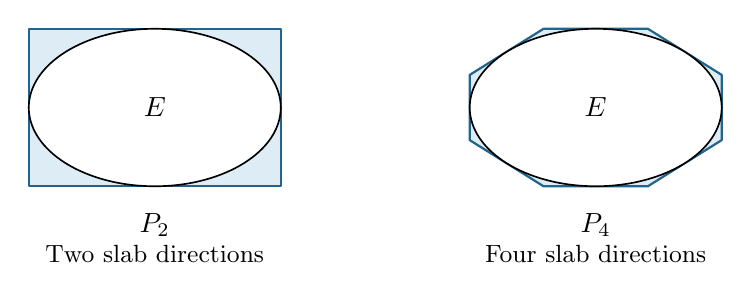
\begin{tikzpicture}[x=1cm,y=1cm,line join=round]
    \definecolor{slabblue}{RGB}{34,100,139}
    \definecolor{slabfill}{RGB}{222,237,245}
    \begin{scope}[xshift=-2.8cm]
      \filldraw[fill=slabfill,draw=slabblue,line width=0.8pt]
        (-1.6,-1) rectangle (1.6,1);
      \filldraw[fill=white,draw=black,line width=0.6pt]
        (0,0) ellipse [x radius=1.6,y radius=1];
      \node at (0,0) {$E$};
      \node[anchor=north] at (0,-1.22) {$P_2$};
      \node[anchor=north,font=\small] at (0,-1.62)
        {Two slab directions};
    \end{scope}
    \begin{scope}[xshift=2.8cm]
      \foreach \k in {0,...,7} {
        \coordinate (p\k) at
          ({1.6*cos(22.5+45*\k)/cos(22.5)},
           {sin(22.5+45*\k)/cos(22.5)});
      }
      \filldraw[fill=slabfill,draw=slabblue,line width=0.8pt]
        (p0) \foreach \k in {1,...,7} {-- (p\k)} -- cycle;
      \filldraw[fill=white,draw=black,line width=0.6pt]
        (0,0) ellipse [x radius=1.6,y radius=1];
      \node at (0,0) {$E$};
      \node[anchor=north] at (0,-1.22) {$P_4$};
      \node[anchor=north,font=\small] at (0,-1.62)
        {Four slab directions};
    \end{scope}
  \end{tikzpicture}
  \caption{Finite outer approximations of an ellipse $E$. Adding slab
  directions gives $P_2\supset P_4\supset E$; the subscripts here count
  slab directions. Using nested finite spanning direction
  sets with dense union, the same construction recovers $\mathcal W[f]$ from any
  positive continuous even function $f$ on the sphere; $f$ need not be a
  support function.}
  \label{fig:slab-exhaustion}
\end{figure}


Figure~\ref{fig:slab-exhaustion} illustrates how additional slab
directions refine an outer approximation.  To pass to all directions,
let $K,L$ be as in Theorem~\ref{thm:main}. Choose nested finite
sets $D_m\subset S^{n-1}$ that contain the coordinate vectors and
whose union is dense in the sphere. Define
\[
 P_m(t)=\bigcap_{p\in D_m}
 \{x:|\langle p,x\rangle|\le h_K(p)^{1-t}h_L(p)^t\}.
\]
The bodies $P_m(t)$ decrease with $m$ and are all contained in the bounded
body $P_1(t)$. By continuity of the support functions and their
evenness,
\[
 \bigcap_m P_m(t)=\mathcal W[h_K^{1-t}h_L^t].
\]
Indeed any point satisfying the dense set of inequalities satisfies
all of them by continuity in the direction. Conversely, the Wulff
inequalities imply the absolute-value constraints by evenness.
At $t=0,1$ these intersections are $K,L$, respectively, by the
supporting-half-space characterization of a convex body.
Continuity of measure from above, applied at $0,\lambda,1$ in
\eqref{eq:slabs}, proves \eqref{eq:main}.

Finally, in dimension one write $K=[-a,a]$ and $L=[-b,b]$ with
$a,b>0$. Their Wulff interpolation is the interval with radius
$a^{1-\lambda}b^\lambda$, whose length is
$(2a)^{1-\lambda}(2b)^\lambda$. Thus \eqref{eq:main} is equality.
The endpoints $\lambda=0,1$ are equality in every dimension.
\end{proof}

\section{Moment coordinates on the whole space}\label{sec:moment}

The variance argument uses a change of variables whose Jacobian is a
positive Hessian.  The following lemma supplies this change of variables
and the uniform upper bound needed for the later cutoff arguments.

\begin{lemma}[Moment coordinates]\label{lem:moment}
Let $n\ge2$, $\eps>0$, and let $V\in C^\infty(\R^n)$ be even with
$D^2V\ge\eps I$.  Set
\[
 Z=\int_{\R^n}e^{-V(x)}\,dx,
 \qquad d\mu(x)=Z^{-1}e^{-V(x)}\,dx.
\]
There is an even $\varphi\in C^\infty(\R^n)$ such that
$d\nu(z)=e^{-\varphi(z)}\,dz$ is a probability measure,
$\nabla\varphi$ is a diffeomorphism of $\R^n$ onto $\R^n$, and
\begin{equation}\label{eq:moment}
 (\nabla\varphi)_\#\nu=\mu,
 \qquad 0<D^2\varphi\le\frac4\eps I,
 \qquad
 \log\det D^2\varphi
   =V(\nabla\varphi)+\log Z-\varphi.
\end{equation}
Moreover, $\varphi(z)\ge c|z|-b$ for some $c>0$ and $b<\infty$.
The lower Hessian bound in \eqref{eq:moment} means positive definiteness
at every point; it need not be uniform on $\R^n$.
\end{lemma}

\begin{proof}
Evenness and uniform convexity give
$V(x)\ge V(0)+\eps|x|^2/2$, so $0<Z<\infty$.
For $R\ge2$, write $B_R=\{x:|x|<R\}$ and set
\[
 Z_R=\int_{B_R}e^{-V(x)}\,dx,
 \qquad d\mu_R=Z_R^{-1}\mathbf1_{B_R}e^{-V(x)}\,dx.
\]
We first use two compact-support results.  The moment theorem of
Berman--Berndtsson \cite[Theorem~1.1]{BermanBerndtsson2013}, applied to
the body $\overline B_R$ and the positive smooth density
$e^{-V}/Z_R$, gives a smooth convex potential $\varphi_R$, unique up to
translation, for which $\nabla\varphi_R:\R^n\to B_R$ is a
diffeomorphism and
\begin{equation}\label{eq:moment-truncated}
 \det D^2\varphi_R
   =Z_R\exp\{V(\nabla\varphi_R)-\varphi_R\}.
\end{equation}
The centering hypothesis holds by evenness.  Integrating the equation
through this diffeomorphism shows that
$d\nu_R=e^{-\varphi_R}\,dz$ is a probability and
$(\nabla\varphi_R)_\#\nu_R=\mu_R$.
Klartag's estimate \cite[Proposition~3.1 and Remark~3.5]{KlartagArxiv2013}
gives
\[
 0<D^2\varphi_R\le CI,\qquad C=4/\eps.
\]
Indeed, the ball has smooth positively curved boundary, and
$\rho_R=V+\log Z_R$ is convex and smooth, with itself and all its
derivatives bounded on $B_R$, and $D^2\rho_R\ge\eps I$.
The constant $C$ is independent of $R$.

Translate the unique preimage of $0$ to $0$.  It is the unique minimum
of $\varphi_R$.  Reflection gives a second potential for the same
target with its minimum at $0$; uniqueness up to translation therefore
makes $\varphi_R$ even.  For each fixed $R$, take the preimages of
the slopes $\pm(R/2)e_i$.  Their supporting planes give
\[
 \varphi_R(z)\ge\frac{R}{2\sqrt n}|z|-b_R
\]
with a finite, possibly $R$-dependent constant $b_R$.
Thus $\nu_R$ has an exponential tail.  In particular, since
$|\nabla\varphi_R|\le R$, integration of
$\operatorname{div}(z e^{-\varphi_R})$ with expanding compact cutoffs
is justified and yields
\begin{equation}\label{eq:moment-source-identity}
 \E_{\nu_R}\,z\cdot\nabla\varphi_R(z)=n.
\end{equation}

We now obtain bounds independent of $R$.  Put
$m_R=\varphi_R(0)$ and $g_R=\varphi_R-m_R\ge0$.
The Hessian bound implies
$g_R(y)\le C|y|^2/2$ and $|\nabla\varphi_R(y)|\le C|y|$.
For arbitrary $y,z$, set $x=\nabla\varphi_R(z)$.  Supporting planes
at $z$ and $-z$ give the single pointwise inequality
\[
 g_R(y)\ge g_R(z)+|x\cdot y|-x\cdot z.
\]
Integrate with respect to $\nu_R$, discard the nonnegative
$\E_{\nu_R}g_R$, and use \eqref{eq:moment-source-identity}:
\[
 g_R(y)\ge\int|x\cdot y|\,d\mu_R(x)-n.
\]
On $B_1$ the density of $\mu_R$ is at least
$d_0=Z^{-1}\exp(-\max_{\overline B_1}V)>0$.
Rotational symmetry of the ball therefore bounds the integral below
by $c|y|$, where $c=d_0\int_{B_1}|x_1|\,dx>0$.  Hence
\begin{equation}\label{eq:moment-coercivity}
 c|y|-n\le g_R(y)\le\frac C2|y|^2,
 \qquad
 \left(\frac{2\pi}{C}\right)^{n/2}
 \le e^{m_R}=\int e^{-g_R(y)}\,dy
 \le e^n\int e^{-c|y|}\,dy.
\end{equation}
This bounds $m_R$ on both sides and gives one integrable exponential
majorant for all the densities $e^{-\varphi_R}$.

It remains to obtain a smooth limit and to verify that its gradient
reaches every point.  On each fixed ball, the preceding estimates
bound $\varphi_R$ and $\nabla\varphi_R$ uniformly.  Since
$Z_2\le Z_R\le Z$, equation \eqref{eq:moment-truncated} bounds
$\det D^2\varphi_R$ below by a positive constant there.
Together with $D^2\varphi_R\le CI$, this gives a uniform local bound
$\delta I\le D^2\varphi_R\le CI$: if the determinant is at least
$d>0$, every eigenvalue is at least $d/C^{n-1}$.
The right-hand sides
\[
 f_R=V(\nabla\varphi_R)+\log Z_R-\varphi_R
\]
of the logarithmic equations are uniformly Lipschitz on that ball,
because
$\nabla f_R=D^2\varphi_R\nabla V(\nabla\varphi_R)
-\nabla\varphi_R$ is uniformly bounded.

To apply an interior uniformly elliptic estimate, choose a smooth
concave scalar function $s$ equal to $\log$ on a slightly larger
interval than $[\delta,C]$, with $s'$ bounded above and bounded below
by positive constants on $\R$.  Such an extension is obtained by
smoothly continuing the decreasing derivative $1/t$ to positive
constant tails.  For symmetric matrices $Q$, the spectral function
$\mathcal F(Q)=\tr s(Q)$ is smooth, concave and uniformly elliptic:
its derivative has eigenvalues $s'(\lambda_i(Q))$, and its second
variation has coefficients $s''(\lambda_i)$ and the nonpositive
divided differences of $s'$.  It agrees with $\log\det$ on the
Hessians under consideration.  The nonhomogeneous Evans--Krylov
estimate \cite[Corollary~2.3]{Wang2012} applied to
$\mathcal F(D^2\varphi_R)=f_R$ gives uniform interior
$C^{2,\alpha}$ bounds for some $\alpha>0$.

Each $\varphi_R$ is already smooth.  Its derivative
$w_{R,k}=\partial_k\varphi_R$ satisfies
\[
 (D^2\varphi_R)^{-1}:D^2w_{R,k}
   =\nabla V(\nabla\varphi_R)\cdot\nabla w_{R,k}-w_{R,k},
\]
where $Q:N=\tr(Q^TN)$.  The principal coefficients and the
right-hand side are uniformly $C^\alpha$ on smaller balls.
Interior Schauder estimates
\cite[Theorem~2.20 and Corollary~2.21]{FernandezRealRosOton2023}
give uniform $C^{3,\alpha}$ bounds for $\varphi_R$, and iteration
gives bounds for every derivative on compact sets.
A diagonal subsequence, still indexed by $R$, converges locally smoothly to an even
$\varphi$ with positive definite Hessian, the same upper cap, and
the logarithmic equation in \eqref{eq:moment}.
The bound $\varphi_R(z)\ge c|z|-b$, with $b$ independent of $R$,
also passes to $\varphi$.

The common exponential majorant from \eqref{eq:moment-coercivity}
proves $\int e^{-\varphi}=1$ by dominated convergence.  For each
bounded continuous $h$, it also gives
\[
 \int h(\nabla\varphi)e^{-\varphi}
 =\lim_{R\to\infty}\int h(\nabla\varphi_R)e^{-\varphi_R}
 =\lim_{R\to\infty}\int h\,d\mu_R
 =\int h\,d\mu.
\]
Thus $(\nabla\varphi)_\#\nu=\mu$.
Positive definite Hessian makes the gradient locally invertible and
injective, since for $z\ne w$,
\[
 (\nabla\varphi(z)-\nabla\varphi(w))\cdot(z-w)
 =\int_0^1 D^2\varphi(w+t(z-w))[z-w,z-w]\,dt>0.
\]
Its image is dense: an open ball missed by the image would have zero
pushforward mass, contrary to the everywhere positive density of
$\mu$.  Fix $x_0\in\R^n$.  Density permits finitely many image
points $y_j=\nabla\varphi(z_j)$ whose convex hull contains a ball
$B_r(x_0)$ with $r>0$; one may take small perturbations of the
points $x_0\pm e_i$.  Their supporting planes imply
\[
 \varphi(z)-x_0\cdot z
 \ge\max_j\{(y_j-x_0)\cdot z+\varphi(z_j)-y_j\cdot z_j\}
 \ge r|z|-b_{x_0}.
\]
This function attains a minimum, at which
$\nabla\varphi=x_0$.  The gradient is therefore onto, and its local
smooth inverses combine to a global smooth inverse.
\end{proof}

We will write $x=\nabla\varphi(z)$ and
$\tau=D_z^2\varphi$, evaluating $\tau$ at the corresponding point
when using $x$ coordinates.  Thus
$\tau(x)=D_z^2\varphi((\nabla\varphi)^{-1}(x))$ is smooth, even,
positive definite and bounded above by $(4/\eps)I$.
The gradient is odd, as is its inverse.  Finally, a compactly
supported smooth function of $x$ is compactly supported after
composition with $\nabla\varphi$: its support lies in the image of
a compact set under the continuous inverse map.  Consequently the
compact integrations by parts below are valid in either coordinate
system.

\section{Adjoints in moment coordinates}\label{sec:identities}

We retain the probability measures
\[
 d\mu(x)=Z^{-1}e^{-V(x)}\,dx,
 \qquad d\nu(z)=e^{-\varphi(z)}\,dz,
 \qquad x=\nabla\varphi(z),
\]
and the smooth diffeomorphism constructed above.  Put
\[
 \tau=D_z^2\varphi,\qquad M=\tau^{-1}.
\]
In target coordinates, these symbols denote the same matrix fields
evaluated at $z=(\nabla\varphi)^{-1}(x)$.
Expectation under either measure, with functions identified by this map,
is denoted by $\E$.
Throughout the coordinate calculations, repeated indices are summed
from $1$ to $n$, and $Q:L=\tr(Q^TL)$ denotes matrix contraction.

We first construct the compact test functions used in the variance
argument and establish an identity that will also identify the
obstruction to their density.  Write
\[
 \partial_k=\partial_{z_k},\qquad
 \partial_k^*=x_k-\partial_k.
\]
The latter is the adjoint of $\partial_k$ in $L^2(\nu)$ because
$\partial_k\varphi=x_k$.  In target coordinates, write $\delta_\mu$
for negative weighted divergence:
\[
 \delta_\mu W
 =\sum_j\bigl(V_{x_j}W_j-\partial_{x_j}W_j\bigr).
\]
On a matrix, $\delta_\mu$ acts on each row, producing a vector.
For a smooth row field $P_{ak}$ and a compact test $g$, the chain rule
and adjunction give
\[
 \E g\,\partial_k^*P_{ak}
 =\E(\partial_k g)P_{ak}
 =\E g_{x_i}\tau_{ik}P_{ak}.
\]
Consequently
\begin{equation}\label{eq:row-adjoint}
 \partial_k^*P_{ak}=(\delta_\mu(P\tau))_a.
\end{equation}
Taking $P$ to be the identity matrix also gives $\delta_\mu\tau=x$.
This is Fathi's moment-map construction of a Stein kernel
\cite[Theorem~2.3 of the cited arXiv version]{Fathi2019}: the matrix
field $\tau$ expresses integration by parts against $x$ through
$\E x_j g=\E\tau_{jk}g_{x_k}$.

Thus the differential operator
\begin{equation}\label{eq:operator-A}
 Af=\delta_\mu(\tau\nabla_x f)
   =\partial_k^*f_{x_k}
   =x\cdot\nabla_x f-\tau:D_x^2f
\end{equation}
is formally symmetric, with
\begin{equation}\label{eq:A-form}
 \E gAf=\E\nabla_xg\cdot\tau\nabla_xf
\end{equation}
for compact smooth tests.  These formulas involve no operator-domain
assertion. This is the negative of the moment-Hessian diffusion
generator studied by Klartag \cite[Section~6]{KlartagArxiv2013};
for our sign convention, $Ax_j=x_j$.

For $f\in C_c^\infty(\R_x^n)$, define
\begin{equation}\label{eq:test-fields}
 h=D_x^2f,\qquad P=\tau h,\qquad B=\tau h\tau,
 \qquad W_a=\partial_k^*P_{ak},\qquad u=\delta_\mu W.
\end{equation}
All these fields have compact support in both coordinates: the inverse
image of a compact target set is its compact image under the continuous
inverse diffeomorphism.  By \eqref{eq:row-adjoint},
$W=\delta_\mu B$.  For every smooth function $F$ in target coordinates,
two adjunctions give
\begin{equation}\label{eq:test-pairing}
 \E uF=\E W\cdot\nabla_xF=\E B:D_x^2F.
\end{equation}
The fields are compactly supported, so $F$ need not be.
Thus the same pairing can be estimated through either the first or the
second derivatives of $F$.
To identify the range of these tests, we also use the gradient identity
\begin{equation}\label{eq:W-gradient}
 W=\nabla_z\bigl[((A-1)f)(x(z))\bigr]
   =\tau\nabla_x(A-1)f,
 \qquad u=A(A-1)f.
\end{equation}
To check it directly, put
$C_{ijk}=\partial_{z_i}\partial_{z_j}\partial_{z_k}\varphi$.
This tensor is fully symmetric, and expansion gives
\[
 W_a=x_k\tau_{ai}f_{x_ix_k}
       -C_{aik}f_{x_ix_k}
       -\tau_{ai}\tau_{jk}f_{x_ix_kx_j}.
\]
Differentiating $(A-1)f$ in $z_a$ gives exactly these terms: the
first-gradient terms from $x\cdot\nabla_xf$ and $-f$ cancel.
The formula for $u$ follows from \eqref{eq:operator-A}.
In particular, $D_zW$ is symmetric.

The following identity is the moment-coordinate specialization of
the transport-Hessian Bochner formula of Kolesnikov, Livshyts and
Rotem \cite[Proposition~4.8]{KLR2026}. We give its direct derivation
in the present notation. Two compact integrations by parts give
\begin{equation}\label{eq:hessian}
 \begin{aligned}
 \E(Af)(A-1)f
 &=\E\nabla_x f\cdot\tau\nabla_x(A-1)f
   =\E\nabla_x f\cdot W\\
 &=\E h:B
   =\E\bigl\|\tau^{1/2}D_x^2f\,\tau^{1/2}\bigr\|_{\mathrm{HS}}^2.
 \end{aligned}
\end{equation}
Here $\|Q\|_{\mathrm{HS}}^2=\tr(Q^TQ)$.
The differential expression $A$ satisfies $A1=0$ and $Ax_j=x_j$,
so $A(A-1)$ annihilates every affine function.
Section~\ref{sec:density} uses \eqref{eq:hessian} to prove that these
are the only $L^2$ obstructions to density. Centering removes constants,
and evenness removes linear functions.

\section{Density of the even tests}\label{sec:density}

The Hessian identity identifies affine functions as the possible
obstructions to density.  We now show that these are the only
obstructions, using cutoffs in the $x$ coordinates.

\begin{lemma}[Density of even tests]\label{lem:density}
Let $d\mu=\rho(x)\,dx$ be a probability measure on $\R^n$ with a smooth,
strictly positive, even density.  Let $\tau$ be a smooth even symmetric
matrix field with $0<\tau(x)\le\Lambda I$ for some finite $\Lambda$, and set
\[
 Af=x\cdot\nabla f-\tau:D^2f.
\]
Suppose that $A$ has the integration formula
\[
 \E[hAf]=\E[\nabla h\cdot\tau\nabla f]
 \qquad(f,h\in C_c^\infty(\R^n))
\]
and satisfies the compact Hessian identity~\eqref{eq:hessian}.
Then
\[
 \overline{\{A(A-1)f:f\in C_c^\infty(\R^n),\ f\text{ even}\}}^{\,L^2(\mu)}
 =\{g\in L^2(\mu):g\text{ even},\ \E g=0\}.
\]
\end{lemma}

\begin{proof}
Write $\Gamma(f,h)=\nabla f\cdot\tau\nabla h$ and
$\Gamma(f)=\Gamma(f,f)$.  The integration formula also holds when one
factor is smooth and the other has compact support, by inserting a
cutoff around that support.  In particular $\E Ak=0$ for compactly
supported smooth $k$.  Since $A$ preserves parity, the displayed range
consists of centered even functions.

Let $g$ be a centered even $L^2(\mu)$ function orthogonal to this range.
It also annihilates $A(A-1)f$ for odd $f$, because that image is odd.
Formal symmetry therefore gives
\[
 \mathcal P g=0\quad\text{in distributions},\qquad \mathcal P=A(A-1).
\]
Indeed, if $\mathcal P^t$ denotes the transpose with respect to
Lebesgue measure and $d\mu=\rho\,dx$, weighted formal symmetry gives
$\mathcal P^t(\rho g)=\rho\mathcal P g$ in distributions.
Orthogonality makes the left side zero, and smooth positivity of
$\rho$ gives the displayed equation.  The principal symbol of $\mathcal P$ is
$(\xi\cdot\tau(x)\xi)^2$, which is positive for every $\xi\ne0$.
Interior elliptic regularity consequently gives $g\in C^\infty$
\cite[Theorem~14.2]{Dyatlov2026}.  Only positivity on compact sets is
needed here.

\smallskip
\noindent\emph{Splitting the equation in $L^2$.}
Choose $0\le\eta_r\le1$ smooth, equal to one on $B_r$, zero outside
$B_{2r}$, with $|\nabla\eta_r|\le C/r$ and $|D^2\eta_r|\le C/r^2$,
where $r\ge1$.  The upper bound on $\tau$ gives constants $B,K$,
independent of $r$, such that
\begin{equation}\label{eq:density-cutoff}
 \Gamma(\eta_r)^{1/2}\le B/r,
 \qquad |A\eta_r|\le K.
\end{equation}
For the second estimate, use $|x|\le2r$ on the support of the cutoff
derivatives.  Those derivatives, including $A\eta_r$, vanish outside
$B_{2r}\setminus B_r$.

Put $v=Ag$, initially just a smooth function, and write
\[
 G=\|g\|_2,\qquad
 X_r=\|\eta_r^2v\|_2,\qquad
 Y_r^2=\E[\eta_r^2\Gamma(g)].
\]
Here $G$ is finite by hypothesis, while $X_r,Y_r$ are finite by compact
support.
Testing $\mathcal P g=0$ against $\eta_r^4g$ gives
$\E[v(A-1)(\eta_r^4g)]=0$.
The product rule $A(ab)=aAb+bAa-2\Gamma(a,b)$ yields the exact expansion
\[
 \begin{split}
 (A-1)(\eta_r^4g)
 ={}&\eta_r^4v
 +g\bigl(4\eta_r^3A\eta_r-12\eta_r^2\Gamma(\eta_r)-\eta_r^4\bigr)\\
 &-8\eta_r^3\Gamma(\eta_r,g).
 \end{split}
\]
Thus Cauchy--Schwarz and~\eqref{eq:density-cutoff} imply
\begin{equation}\label{eq:density-two-estimates}
 X_r\le aG+\frac{8B}{r}Y_r,
 \qquad
 Y_r^2\le GX_r+\frac{2B}{r}GY_r,
 \qquad a=1+4K+12B^2.
\end{equation}
The first inequality is immediate if $X_r=0$; otherwise divide the
resulting estimate for $X_r^2$ by $X_r$.  For the second, integrate by
parts in $\E[\eta_r^2gAg]$:
\[
 Y_r^2=\E[\eta_r^2gv]-2\E[\eta_rg\Gamma(\eta_r,g)].
\]
Combining~\eqref{eq:density-two-estimates} gives
$Y_r^2\le aG^2+10BGY_r$, so both $Y_r$ and $X_r$ are bounded uniformly
in $r$.  Exhaustion by balls proves $v=Ag\in L^2(\mu)$.  We may now set
\[
 w=g-v\in L^2(\mu),\qquad Aw=0,\qquad Av=v.
\]

\smallskip
\noindent\emph{The harmonic part is constant.}
Testing $Aw=0$ with $\eta_r^2w$ and using
\eqref{eq:density-cutoff} gives
\[
 \bigl(\E[\eta_r^2\Gamma(w)]\bigr)^{1/2}
 \le\frac{2B}{r}\|w\|_2.
\]
On any fixed ball, let $r\to\infty$.  Then $\Gamma(w)=0$ there;
strict positivity of $\tau$ shows that $w$ is constant.

\smallskip
\noindent\emph{The eigenvalue-one part is linear.}
The analogous test of $Av=v$ gives, with
$Z_r^2=\E[\eta_r^2\Gamma(v)]$,
\[
 Z_r^2\le\|v\|_2^2+\frac{2B}{r}\|v\|_2Z_r.
\]
Hence $\E\Gamma(v)<\infty$.  For $f_r=\eta_rv\in C_c^\infty$,
the product rule now proves directly that
\begin{equation}\label{eq:density-approximation}
 f_r\longrightarrow v,\qquad Af_r\longrightarrow v
 \quad\text{in }L^2(\mu).
\end{equation}
Indeed,
\[
 Af_r=\eta_rv+vA\eta_r-2\Gamma(\eta_r,v).
\]
The middle term has norm at most
$K\|v\mathbf{1}_{B_{2r}\setminus B_r}\|_2\to0$.  For the last term, use
\[
 \|\Gamma(\eta_r,v)\|_2
 \le\frac{B}{r}(\E\Gamma(v))^{1/2}\longrightarrow0.
\]
Apply~\eqref{eq:hessian} to these compactly supported functions:
\[
 \E\bigl[\|\tau^{1/2}D^2f_r\,\tau^{1/2}\|_{\mathrm{HS}}^2\bigr]
 =\|Af_r\|_2^2-\E[f_rAf_r]\longrightarrow0.
\]
On each fixed ball, $f_r=v$ for all sufficiently large $r$.  Positivity
of the density and of $\tau$ therefore forces $D^2v=0$ on that ball.
Thus $v$ is affine, and $Av=v$ removes its constant term.

We have proved that every $L^2$ distributional solution of $\mathcal P g=0$ is
affine.  Our $g=w+v$ is even, so it is constant, and its mean is zero.
Hence $g=0$.  Taking the orthogonal complement in the centered even
subspace proves the lemma.
\end{proof}

\section{A tensor estimate for the divergence tests}\label{sec:tensor}

The gradient and Hessian pairings in \eqref{eq:test-pairing} will be
estimated using two quadratic energies, one for $W$ and one for $B$.
The following lemma bounds their sum by $\E u^2$. Its proof uses weighted
integration by parts and the moment equation; homogeneity enters only
when the lemma is applied to the summands $\psi_i$ in
Section~\ref{sec:variance}.

\begin{lemma}[Moment-coordinate tensor estimate]\label{lem:tensor}
Let $d\mu=Z^{-1}e^{-V}dx$ and $d\nu=e^{-\varphi}dz$ be smooth
probability measures on $\R^n$.  Suppose $D_z^2\varphi$ is positive
definite and $x=\nabla\varphi(z)$ is a smooth diffeomorphism pushing
$\nu$ to $\mu$.
For a real $f\in C_c^\infty(\R_x^n)$, put
\[
 \tau=D_z^2\varphi,\quad M=\tau^{-1},\quad H=D_x^2V,
 \quad B=\tau(D_x^2f)\tau,
 \quad W=\delta_\mu B,
 \quad u=\delta_\mu W.
\]
View source fields in target coordinates by the inverse moment map.
Then
\begin{equation}\label{eq:tensor-estimate}
 \E\tr\bigl((D_xW)^2\bigr)
 \ge \E\tr(MBHB),
\end{equation}
and
\begin{equation}\label{eq:tensor-energy}
 \E u^2\ge\E\tr(MBHB)+\E W^THW.
\end{equation}
Here $(D_xW)_{ij}=\partial_{x_j}W_i$, and the square in
\eqref{eq:tensor-estimate} is a matrix square.
\end{lemma}

\begin{proof}
All test fields used in the integrations by parts below have compact support.
Weighted Bochner calculations underlie many variance estimates; see
Bakry--\'Emery \cite[Proposition~3]{BakryEmery1985} and the
transport-Hessian formulas in \cite[Section~4.3]{KLR2026}.
Here the required identity is for a vector field, so we derive it
explicitly and retain the matrix trace $\tr((D_xW)^2)$.
First, for any such vector field $W$ and $u=\delta_\mu W$,
\[
 \partial_{x_i}u
 =H_{ij}W_j+(V_{x_j}-\partial_{x_j})\partial_{x_i}W_j.
\]
Pairing with $W_i$ and using adjunction gives the weighted identity
\begin{equation}\label{eq:bochner}
 \E u^2
 =\E W_i\partial_{x_i}u
 =\E W^THW
   +\E(\partial_{x_j}W_i)(\partial_{x_i}W_j)
 =\E W^THW+\E\tr\bigl((D_xW)^2\bigr).
\end{equation}
Thus it remains to prove \eqref{eq:tensor-estimate}.
Its proof compares two expansions, integrates their derivative terms
by parts, and writes the resulting difference as a sum of squares.

Recall $h=D_x^2f$ and $P=\tau h$ from \eqref{eq:test-fields}, and let
$(C_i)_{kl}=C_{ikl}$, where $C=D_z^3\varphi$.
The moment equation \eqref{eq:moment} reads
\[
 V(x(z))=\varphi(z)+\log\det\tau(z)-\log Z.
\]
Its first derivative gives
\[
 \tau_{ik}V_{x_k}=x_i+c_i,
 \qquad c_i=\tr(MC_i).
\]
Since $\partial_jM=-MC_jM$, differentiating once more gives
\[
 (\tau H\tau)_{ij}
 =\tau_{ij}+M_{kl}\varphi_{klij}
   -\tr(MC_iMC_j)-C_{ijk}V_{x_k}.
\]
To combine the fourth-derivative term and the term involving
$\nabla_xV$ into a weighted divergence, note that
\[
 \partial_dM_{dk}
 =-M_{da}C_{abd}M_{bk}=-c_bM_{bk},
 \qquad
 \partial_dM_{dk}-x_dM_{dk}=-V_{x_k}.
\]
Full symmetry of $D_z^4\varphi$ therefore yields
\begin{equation}\label{eq:twice-moment}
 (\tau H\tau-\tau)_{ij}
 =(\partial_d-x_d)(M_{dk}C_{ijk})
   -\tr(MC_iMC_j).
\end{equation}

For the other expansion, the commutator
$[\partial_l,\partial_k^*]=\tau_{kl}$ gives
\[
 D_zW=B+R,\qquad R_{al}=\partial_k^*\partial_lP_{ak}.
\]
Both $D_zW$ and $B$ are symmetric, so $R$ is symmetric.
Since $D_xW=(B+R)M$ and $MBM=h$, expansion followed by one
integration by parts gives
\begin{equation}\label{eq:trace-expansion}
 \E\tr\bigl((D_xW)^2\bigr)
 =\E\tr(MBMB)
  +2\E(\partial_kh_{al})(\partial_lP_{ak})
  +\E\tr(MRMR).
\end{equation}
The last term is nonnegative:
$\tr(MRMR)=\|M^{1/2}RM^{1/2}\|_{\mathrm{HS}}^2$.
On the right side of \eqref{eq:tensor-estimate}, the coefficient of
$\tau H\tau$ in the trace contraction is
\[
 Q=MBMBM=h\tau h.
\]
Substituting \eqref{eq:twice-moment} and integrating its divergence
term by parts gives
\begin{equation}\label{eq:H-expansion}
 \E\tr(MBHB)
 =\E\tr(MBMB)
   -\E(\partial_dQ_{ij})M_{dk}C_{ijk}
   -\E Q_{ij}\tr(MC_iMC_j).
\end{equation}
The common first term cancels.  We now evaluate the three remaining
contracted terms in coordinates where $\tau=I$ at the point under
consideration.

This normalization uses a constant dual change of coordinates.
For an invertible constant matrix $T$, set
\[
 z=Tz',\qquad x'=T^Tx,\qquad
 f'(x')=f(T^{-T}x').
\]
The corresponding normalized potentials and partition function are
\[
 \varphi'(z')=\varphi(Tz')-\log|\det T|,
 \qquad V'(x')=V(T^{-T}x'),
 \qquad Z'=|\det T|Z.
\]
They preserve both probability measures by change of variables,
$x'=\nabla_{z'}\varphi'$, and the moment equation.  The chain rule gives
\[
 \begin{array}{lll}
 \tau'=T^T\tau T,& B'=T^TBT,& R'=T^TRT,\\
 M'=T^{-1}MT^{-T},& h'=T^{-1}hT^{-T},& H'=T^{-1}HT^{-T},\\
 Q'=T^{-1}QT^{-T},& P'=T^TPT^{-T},& W'=T^TW.
 \end{array}
\]
Each $z$-derivative index, including all three indices of $C$,
transforms covariantly with $T$; the same law holds for $\partial_k^*$.
Also $D_{x'}W'=T^T(D_xW)T^{-T}$.
It follows that every contracted scalar in
\eqref{eq:trace-expansion} and \eqref{eq:H-expansion} is invariant.
For example, in
$(\partial_kh_{al})(\partial_lP_{ak})$ each index pairs one
covariant and one contravariant factor.
At a fixed point we may therefore take $T=\tau^{-1/2}$, using
the value of $\tau$ at that point.  All derivatives are computed
under this constant transformation.  No moving frame is
differentiated; the integrations by parts have already been completed.

In these normalized coordinates, put
\[
 S_{ijk}=f_{x_ix_jx_k},\qquad J_{ijk}=h_{ia}C_{ajk}.
\]
The tensor $S$ is fully symmetric, and $J$ is symmetric in its last
two indices.  Write $J^{(12)}_{ijk}=J_{jik}$, and use the Euclidean
tensor norm and inner product in this frame.
The three contractions are
\begin{align}
 2(\partial_kh_{al})(\partial_lP_{ak})
   &=2\|S\|^2+2\langle S,J\rangle,\label{eq:normalized-cross}\\
 (\partial_dQ_{ij})C_{ijd}
   &=2\langle S,J\rangle+\langle J,J^{(12)}\rangle,
       \label{eq:normalized-derivative}\\
 Q_{ij}\tr(C_iC_j)&=\|J\|^2.\label{eq:normalized-cubic}
\end{align}
For \eqref{eq:normalized-cross}, use
$\partial_kh_{al}=S_{alk}$ and
$\partial_lP_{ak}=C_{ail}h_{ik}+S_{akl}$.
For \eqref{eq:normalized-derivative}, differentiating the two factors
$h$ in $Q=h\tau h$ gives the two copies of $\langle S,J\rangle$.
Differentiating its middle factor gives
\[
 \sum_{iabjd}h_{ia}C_{abd}h_{bj}C_{ijd}
 =\sum_d\tr(hC_dhC_d)
 =\langle J,J^{(12)}\rangle.
\]
Finally, \eqref{eq:normalized-cubic} follows by expanding
$Q=h^2$ and the trace, using the full symmetry of $C$.

Thus, apart from the nonnegative $R$ term, the integrand of
\eqref{eq:trace-expansion} minus \eqref{eq:H-expansion} is
\[
 2\|S\|^2+4\langle S,J\rangle
   +\|J\|^2+\langle J,J^{(12)}\rangle.
\]
Full symmetrization of $J$ is
\[
 (\operatorname{Sym}J)_{ijk}
 =\frac{J_{ijk}+J_{jik}+J_{kij}}3.
\]
Its norm satisfies
\[
 \|\operatorname{Sym}J\|^2
 =\frac{\|J\|^2+2\langle J,J^{(12)}\rangle}{3},
 \qquad
 \langle S,\operatorname{Sym}J\rangle=\langle S,J\rangle.
\]
Consequently the preceding integrand equals
\begin{equation}\label{eq:tensor-squares}
 2\|S+\operatorname{Sym}J\|^2
 +\frac16\|J-J^{(12)}\|^2\ge0.
\end{equation}
This pointwise calculation proves \eqref{eq:tensor-estimate};
combining it with \eqref{eq:bochner} proves
\eqref{eq:tensor-energy}.
\end{proof}

For the soft slab potentials, $H$ is the sum of a positive quadratic
part and the positive semidefinite Hessians of the homogeneous
summands.  Lemma~\ref{lem:tensor} will control each summand through
the two terms on the right side of \eqref{eq:tensor-energy}.

\section{The variance inequality}
\label{sec:variance}

We now apply the moment-coordinate estimates to the potential
\eqref{eq:potential}. In this section all expectations are with
respect to its probability $\mu$.

\begin{proof}[Proof of Proposition~\ref{prop:variance}]
The potential is smooth and even, and $D^2V\ge\eps I$.
Lemma~\ref{lem:moment} therefore supplies the moment coordinates,
with $0<\tau\le (4/\eps)I$. Put
\[
 H_i=D_x^2\psi_i,\qquad a_i=\E\psi_i.
\]
Each $H_i$ is positive semidefinite, and $a_i>0$ since $p_i\ne0$
and $\mu$ has positive density everywhere. Homogeneity gives
\begin{equation}\label{eq:homogeneity}
 x\cdot\nabla\psi_i=q\psi_i,
 \qquad H_ix=(q-1)\nabla\psi_i.
\end{equation}
The adjunction identity of Section~\ref{sec:identities} also gives
\begin{equation}\label{eq:mi}
 m_i:=\E\tr(\tau H_i)=\E x\cdot\nabla\psi_i=q a_i.
\end{equation}
To justify it for these noncompact functions, apply
$\E x_j k=\E\tau_{jk}\partial_{x_k}k$ to
$k=\eta_R\partial_{x_j}\psi_i$ and sum in $j$, where $\eta_R$
is a smooth cutoff equal to one on $B_R$ and zero outside $B_{2R}$.
The extra term is bounded in absolute value by
$C R^{-1}\E[|\nabla\psi_i|\mathbf1_{\{|x|\ge R\}}]$, which tends
to zero. The other terms converge because $\tau$ is bounded and
all polynomial moments are finite.

Take an even $f\in C_c^\infty(\R^n)$ and use
\[
 B=\tau D_x^2f\,\tau,\qquad W=\delta_\mu B,
 \qquad u=\delta_\mu W=A(A-1)f,
 \qquad M=\tau^{-1}.
\]
Applying \eqref{eq:test-pairing} to $F=\psi_i$ gives, for each $i$,
\begin{equation}\label{eq:di}
 d_i:=\E u\psi_i=\E W\cdot\nabla\psi_i=\E\tr(BH_i).
\end{equation}
Two Cauchy--Schwarz estimates will give complementary bounds for
these same numbers $d_i$.

First apply the Hilbert--Schmidt Cauchy--Schwarz inequality, including
integration, to the matrix fields
$H_i^{1/2}\tau^{1/2}$ and $H_i^{1/2}B\tau^{-1/2}$. Their pairing
is $\tr(H_iB)$, so
\begin{equation}\label{eq:first-cs}
 d_i^2\le m_i\,\E\tr(MBH_iB).
\end{equation}
This does not require $B$ to be positive semidefinite.
Second, \eqref{eq:homogeneity}--\eqref{eq:di} give
\[
 \E x^TH_i x=(q-1)m_i,
 \qquad \E x^TH_iW=(q-1)d_i.
\]
Cauchy--Schwarz for the positive semidefinite form
$(X,Y)\mapsto\E X^TH_iY$ therefore yields
\begin{equation}\label{eq:second-cs}
 \E W^TH_iW\ge(q-1)\frac{d_i^2}{m_i}.
\end{equation}

Since $H=D^2V=\eps I+\sum_iH_i$, Lemma~\ref{lem:tensor} and
the weighted Bochner identity \eqref{eq:bochner} imply
\begin{align}
 \E u^2
 &\ge\E\tr(MBHB)+\E W^THW\notag\\
 &\ge\sum_i\left(\E\tr(MBH_iB)+\E W^TH_iW\right)
 \ge\sum_i\frac{q d_i^2}{m_i}
 =\sum_i\frac{d_i^2}{a_i}.
 \label{eq:dual-bound}
\end{align}
The discarded terms are nonnegative, since $M$ is positive definite
and $B$ is symmetric. This is the required estimate on the dense
class of double divergences.

By Lemma~\ref{lem:density}, such $u$ are dense in the centered even
subspace of $L^2(\mu)$. Each $\psi_i\in L^2(\mu)$, so all pairings
$u\mapsto\E u\psi_i$ are continuous. Thus \eqref{eq:dual-bound}
holds for every centered even $u\in L^2(\mu)$.
For $F=\sum_i b_i\psi_i$, choose $u=F-\E F$. Then
\[
 \|u\|_2^2=\sum_i b_i d_i
 \le\left(\sum_i b_i^2a_i\right)^{1/2}
      \left(\sum_i d_i^2/a_i\right)^{1/2}
 \le\left(\sum_i b_i^2a_i\right)^{1/2}\|u\|_2.
\]
If $\|u\|_2=0$, the conclusion is immediate; otherwise division and
squaring prove \eqref{eq:variance}. This completes the analytic
assertion and, by Section~\ref{sec:reduction}, Theorem~\ref{thm:main}.
\end{proof}

\section{Volume and measure consequences}\label{sec:consequences}

With Theorem~\ref{thm:main} proved, we derive the additive volume
inequality stated in the introduction and then apply Saroglou's
transfer theorem to even log-concave measures.

\subsection{The symmetric \texorpdfstring{$L_p$}{Lp} volume inequality}
\label{subsec:lp-proof}

\begin{proof}[Proof of Corollary~\ref{cor:lp}]
At $\lambda=0,1$, the assertion follows from
$\mathcal W[h_K]=K$ and $\mathcal W[h_L]=L$. Suppose $0<\lambda<1$.
Set
\[
 a=|K|^{1/n}>0,\qquad b=|L|^{1/n}>0,\qquad
 K_0=a^{-1}K,\qquad L_0=b^{-1}L,
\]
so that $|K_0|=|L_0|=1$. Define
\[
 c=\bigl((1-\lambda)a^p+\lambda b^p\bigr)^{1/p}>0,
 \qquad \theta=\frac{\lambda b^p}{c^p}\in(0,1).
\]
Then $1-\theta=(1-\lambda)a^p/c^p$. For every $u\in S^{n-1}$,
the support identities $h_K=a h_{K_0}$ and $h_L=b h_{L_0}$, followed
by the weighted arithmetic--geometric mean inequality, give
\begin{align*}
 \bigl((1-\lambda)h_K(u)^p+\lambda h_L(u)^p\bigr)^{1/p}
 &=c\bigl((1-\theta)h_{K_0}(u)^p+
              \theta h_{L_0}(u)^p\bigr)^{1/p}\\
 &\ge c h_{K_0}(u)^{1-\theta}h_{L_0}(u)^\theta.
\end{align*}
All support values here are positive. The Wulff definition is monotone
in its support bound and satisfies $\mathcal W[cf]=c\mathcal W[f]$ for
$c>0$. Hence
\[
 c\mathcal W[h_{K_0}^{1-\theta}h_{L_0}^\theta]
 \subset
 \mathcal W\!\left[
  \bigl((1-\lambda)h_K^p+\lambda h_L^p\bigr)^{1/p}
 \right].
\]
By Theorem~\ref{thm:main}, the unscaled body on the left has volume at
least $1$, because $K_0,L_0$ are origin-symmetric and have unit volume.
The body on the right therefore has volume at least $c^n$. Raising this
bound to the positive power $p/n$ gives
\eqref{eq:lp}, since $c^p=(1-\lambda)|K|^{p/n}+\lambda|L|^{p/n}$.
\end{proof}

\subsection{Even log-concave measures and the \texorpdfstring{$(B)$}{(B)}-conjecture}
\label{sec:measure}

We now pass from volume to integration against even log-concave measures.
A nonnegative Radon measure $\mu$ on $\R^n$ is \emph{log-concave} if
\[
 \mu((1-\theta)A+\theta B)
 \ge \mu(A)^{1-\theta}\mu(B)^\theta
 \qquad(0<\theta<1)
\]
for all compact sets $A,B\subset\R^n$; it is \emph{even} if
$\mu(A)=\mu(-A)$ for every Borel set $A$. Radon measures are finite on
compact sets, but their total mass need not be finite. We use the analogous
multiplicative definition of log-concavity for nonnegative functions, so
the identically zero function is included. Endpoint products in an
interpolation inequality are understood as the corresponding endpoint
values.

Saroglou's transfer theorem states that the logarithmic Brunn--Minkowski
inequality for Lebesgue measure in a dimension $d$ implies the same
inequality in dimension $d$ for every even log-concave density
\cite[Theorem~3.1]{Saroglou2016}. The density may vanish and need not be
normalized. This theorem is stated for densities with respect to
$d$-dimensional Lebesgue measure. The reduction below makes explicit how
it also gives the measure statement when the measure has lower-dimensional
support.

\begin{corollary}[Measure inequality and scalar $(B)$-conjecture]
\label{cor:measure}
Let $n\ge1$, let $\mu$ be an even log-concave Radon measure on $\R^n$, and
let $K,L\subset\R^n$ be origin-symmetric convex bodies. Then, for every
$0\le\lambda\le1$,
\begin{equation}\label{eq:measure-logbm}
 \mu\bigl(\mathcal W[h_K^{1-\lambda}h_L^\lambda]\bigr)
 \ge \mu(K)^{1-\lambda}\mu(L)^\lambda.
\end{equation}
Consequently, for every origin-symmetric convex body $K\subset\R^n$, the
function
\begin{equation}\label{eq:b-function}
 \R\ni t\longmapsto \mu(e^tK)
\end{equation}
is log-concave.
\end{corollary}

\begin{proof}
Fix $0<\lambda<1$ and write
$D=\mathcal W[h_K^{1-\lambda}h_L^\lambda]$.
The assertion is immediate when $\mu$ is the zero measure. Otherwise,
choose a closed ball $C$ centered at the origin large enough that
$K\cup L\cup D\subset C$ and $0<\mu(C)<\infty$. This is possible because
the three bodies are compact and $\mu$ is a nonzero Radon measure. The
probability measure
\[
 \nu(A)=\frac{\mu(A\cap C)}{\mu(C)}
\]
is even and log-concave: for compact $A,B$, convexity of $C$ gives
\[
 (1-\theta)(A\cap C)+\theta(B\cap C)
 \subset ((1-\theta)A+\theta B)\cap C,
\]
and the defining inequality for $\mu$ applies. Since $K,L,D\subset C$,
the common factor $\mu(C)$ cancels from \eqref{eq:measure-logbm}. It
therefore suffices to prove that inequality for $\nu$.

Let $E$ be the affine hull of $\operatorname{supp}\nu$. Evenness gives
$E=-E$, so $E$ is a linear subspace. If $\dim E=0$, then
$\nu=\delta_0$; all three bodies contain $0$, and equality holds.
Suppose $d=\dim E\ge1$ and identify $E$ isometrically with $\R^d$.
By inner regularity, the compact-set definition
of log-concavity for $\nu$ is equivalent to the Borel-set formulation
using inner measure. Borell's characterization
\cite[Theorem~1.1, with $s=0$]{Borell1974}, applied to $\nu$ on $E$,
represents it as an affine image of a log-concave density in a dimension
$k\le d$. Since its support spans $E$, the affine map has rank $d$.
Thus $k=d$, the map is invertible, and $\nu$ has a log-concave density
$f$ with respect to Lebesgue measure on $E$. Evenness of $\nu$ gives
$f(x)=f(-x)$ almost everywhere; replacing $f(x)$ by
$\sqrt{f(x)f(-x)}$ gives an even log-concave representative of the same
density.

Set $K_E=K\cap E$ and $L_E=L\cap E$. These are origin-symmetric convex
bodies in $E$, since $K$ and $L$ contain neighborhoods of $0$. Define
their relative support functions for every $v\in E$ by
\[
 h^E_{K_E}(v)=\max_{y\in K_E}\langle y,v\rangle,
 \qquad
 h^E_{L_E}(v)=\max_{y\in L_E}\langle y,v\rangle.
\]
The relative Wulff body in $E$ is
\[
 D_E=\bigcap_{v\in E}
 \left\{x\in E:\langle x,v\rangle
 \le h^E_{K_E}(v)^{1-\lambda}h^E_{L_E}(v)^\lambda\right\}.
\]
Using all $v\in E$ rather than only unit vectors gives the same body by
homogeneity. Let $P_E$ be the orthogonal projection onto $E$. For
$x\in D_E$ and $u\in S^{n-1}$,
\begin{align*}
 \langle x,u\rangle
 &=\langle x,P_Eu\rangle\\
 &\le h^E_{K_E}(P_Eu)^{1-\lambda}
       h^E_{L_E}(P_Eu)^\lambda\\
 &\le h_K(u)^{1-\lambda}h_L(u)^\lambda.
\end{align*}
Indeed, $h^E_{K_E}(P_Eu)=\max_{y\in K\cap E}\langle y,u\rangle\le h_K(u)$,
and likewise for $L$; if $P_Eu=0$, the middle product is $0$.
Thus
\begin{equation}\label{eq:relative-wulff-inclusion}
 D_E\subset D\cap E.
\end{equation}
Theorem~\ref{thm:main} in dimension $d$, followed by Saroglou's transfer
theorem \cite[Theorem~3.1]{Saroglou2016} in that same dimension, gives
\[
 \nu(D_E)\ge \nu(K_E)^{1-\lambda}\nu(L_E)^\lambda.
\]
Since $\nu$ is supported on $E$, inclusion
\eqref{eq:relative-wulff-inclusion} yields
\[
 \nu(D)=\nu(D\cap E)\ge\nu(D_E)
 \ge\nu(K)^{1-\lambda}\nu(L)^\lambda,
\]
as required. At $\lambda=0,1$, the Wulff bodies are $K,L$, respectively,
and the endpoint convention gives equality.

Finally, for $s,t\in\R$, the support identity $h_{e^sK}=e^s h_K$ gives
\[
 \mathcal W\!\left[h_{e^sK}^{1-\lambda}h_{e^tK}^\lambda\right]
 =\mathcal W\!\left[e^{(1-\lambda)s+\lambda t}h_K\right]
 =e^{(1-\lambda)s+\lambda t}K.
\]
Applying \eqref{eq:measure-logbm} to $e^sK$ and $e^tK$ proves
\[
 \mu\bigl(e^{(1-\lambda)s+\lambda t}K\bigr)
 \ge \mu(e^sK)^{1-\lambda}\mu(e^tK)^\lambda.
\]
This is exactly the log-concavity in \eqref{eq:b-function}, and is the
scalar-dilation argument of Saroglou \cite[Corollary~3.2]{Saroglou2016}.
\end{proof}


\bibliographystyle{plain}
\bibliography{references}
\end{document}
